\documentclass[tikz]{standalone}
\RequirePackage{luatex85}
\usepackage{tikz}
\usepackage{tkz-euclide}
\usepackage{tkz-tab}
\usepackage{fourier-otf}
\usepackage{fontspec}

\usetikzlibrary{calc}
\usetikzlibrary{3d}
\usepackage{pgfplots}

\tikzset{
  every picture/.append style={scale=2, every node/.style={scale=2}}
}



\begin{document}
  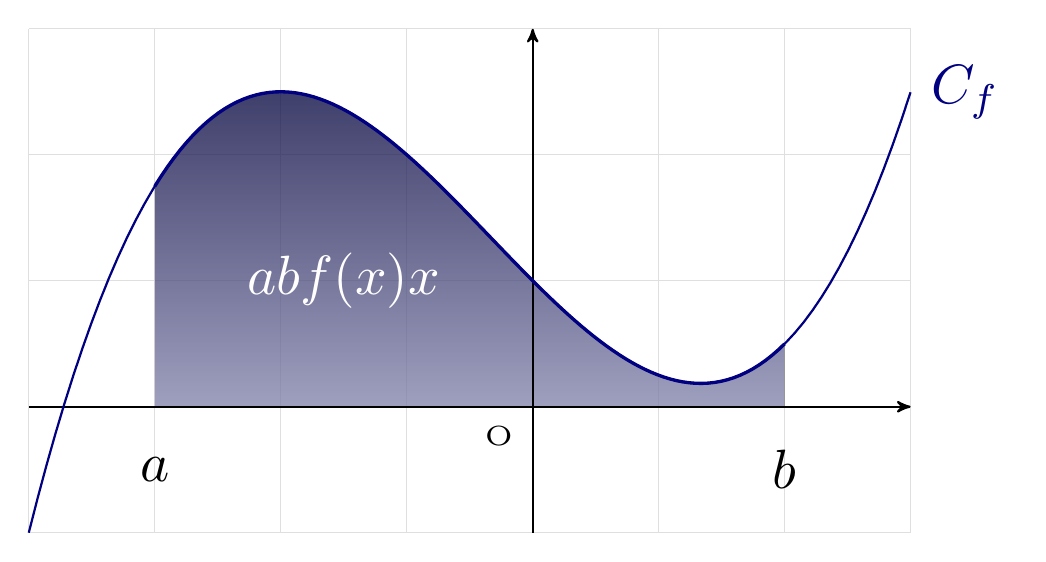
\begin{tikzpicture}[scale=0.8]
\draw[gray!25] (-4,-1) grid (3,3);
\fill[bottom color=blue!25,top color=blue!35!black,opacity=0.5] (-3,0)  plot[domain=-3:2,samples=100] (\x,{0.125*\x*\x*\x+0.125*\x*\x-\x+1}) -- (2,0) -- (-3,0);
\draw[thick,->,>=stealth'] (-4,0) -- (3,0);
\draw[thick,->,>=stealth'] (0,-1) -- (0,3);
\foreach\x in {}
{
	\draw[thick] (\x,0.1) -- (\x,-0.1) node[below] {\tiny\x};
}
\foreach\y in {}
{
	\draw[thick] (-.1,\y) -- (0.1,\y) node[right] {\tiny\y};
}
\node[below left] at (0,0) {\tiny O};
\draw[thick,blue!50!black] plot[domain=-4:3,samples=100] (\x,{0.125*\x*\x*\x+0.125*\x*\x-\x+1}) node[right] {$\mathscr{C}_f$};
\draw[very thick,blue!50!black] plot[domain=-3:2,samples=100] (\x,{0.125*\x*\x*\x+0.125*\x*\x-\x+1});
\node[white] at (-1.5,1) {$ \inte{a}{b}{f(x)}{x}$};
\node  at (-3,-0.5) {$ a $};
\node  at (2,-0.5) {$ b $};
\end{tikzpicture}
\end{document}
